%%%---------------------------------------------------------------%%%
%%% Wyzsza Szkola Gospodarki Bachelor's Thesis                    %%%
%%% Prepared by Bruno Axel Kamere                                 %%%
%%% Inspired by Artur M. Brodzki & Piotr Woźniak's WUT template.  %%%
%%% Computer Engineering and Mechatronics Department              %%%
%%% Wyzsza Szkola Gospodarki w Bydgoszczy, 2022                   %%%
%%%---------------------------------------------------------------%%%
% -------------------------------------------------------------------
% 30. Theory                                                        %
% -------------------------------------------------------------------


%/-------------------------------- CHAPTER START --------------------------------/%

\chapter{Theory}
\label{chap:theory}

In this chapter, key background concepts and methodologies used in the thesis are going to be discussed. The chapter is going to explain what is meant by unmanned aerial system and its components.

The chapter is also going to discuss on the cloud provider, Amazon web services (AWS), used to host various components of developed system, simulation and software development tools used, as well as laws and regulations around unmanned aerial systems.


%/-------------------------------- SECTION START --------------------------------/%

\section{Unmanned Aerial System}
\label{sec:unmanned-aerial-system}

An unmanned aerial system commonly referred to as UAS is a set comprised of an unmanned aerial vehicle (UAV) and components that support its operations. UAVs that make the UAS do not carry human pilots but are piloted remotely or autonomously. A UAS is usually comprised of four main components namely,

\begin{itemize}
    \item An unmanned aerial vehicle also known as a UAV.
    \item A ground control station also known as a GCS, from where human pilots can remotely pilot a UAV or upload mission payload for the UAV to execute autonomously.
    \item Sensors and devices specific to the aerial vehicles' intended mission. These can be cameras or other various sensors.
    \item A data-link between a UAV and a GCS. The data-link can be set up via LTE, WiFi or satellite.
\end{itemize}

A typical UAS also includes some ways to collect telemetry from the UAV to some sort of data-lake for further analysis. The collected data can be used for machine learning to improve the UAV operational efficiency and in building sophisticated operational algorithms.

Figure \ref{fig:solution-hld-a4} shows the high-level design of the proposed unmanned aerial system.


%/------------------------------ SUB-SECTION START ------------------------------/%

\subsection{Unmanned Aerial Vehicle}
\label{subsec:uav}

Unmanned aerial vehicle is a term used to refer to an aerial vehicle that has no human onboard pilot but is rather piloted remotely by humans from a remote ground control station or is autonomously piloted using onboard flight algorithms. Unmanned aerial vehicles are also commonly known as UAVs, drones or remotely piloted vehicles (RPV). A UAV in itself is a system because it is comprised of the multiple components that enable it to fly. Figure \ref{fig:uav-hld} shows a high-level design of the proposed UAV.

\begin{figure}[H]
    \centering 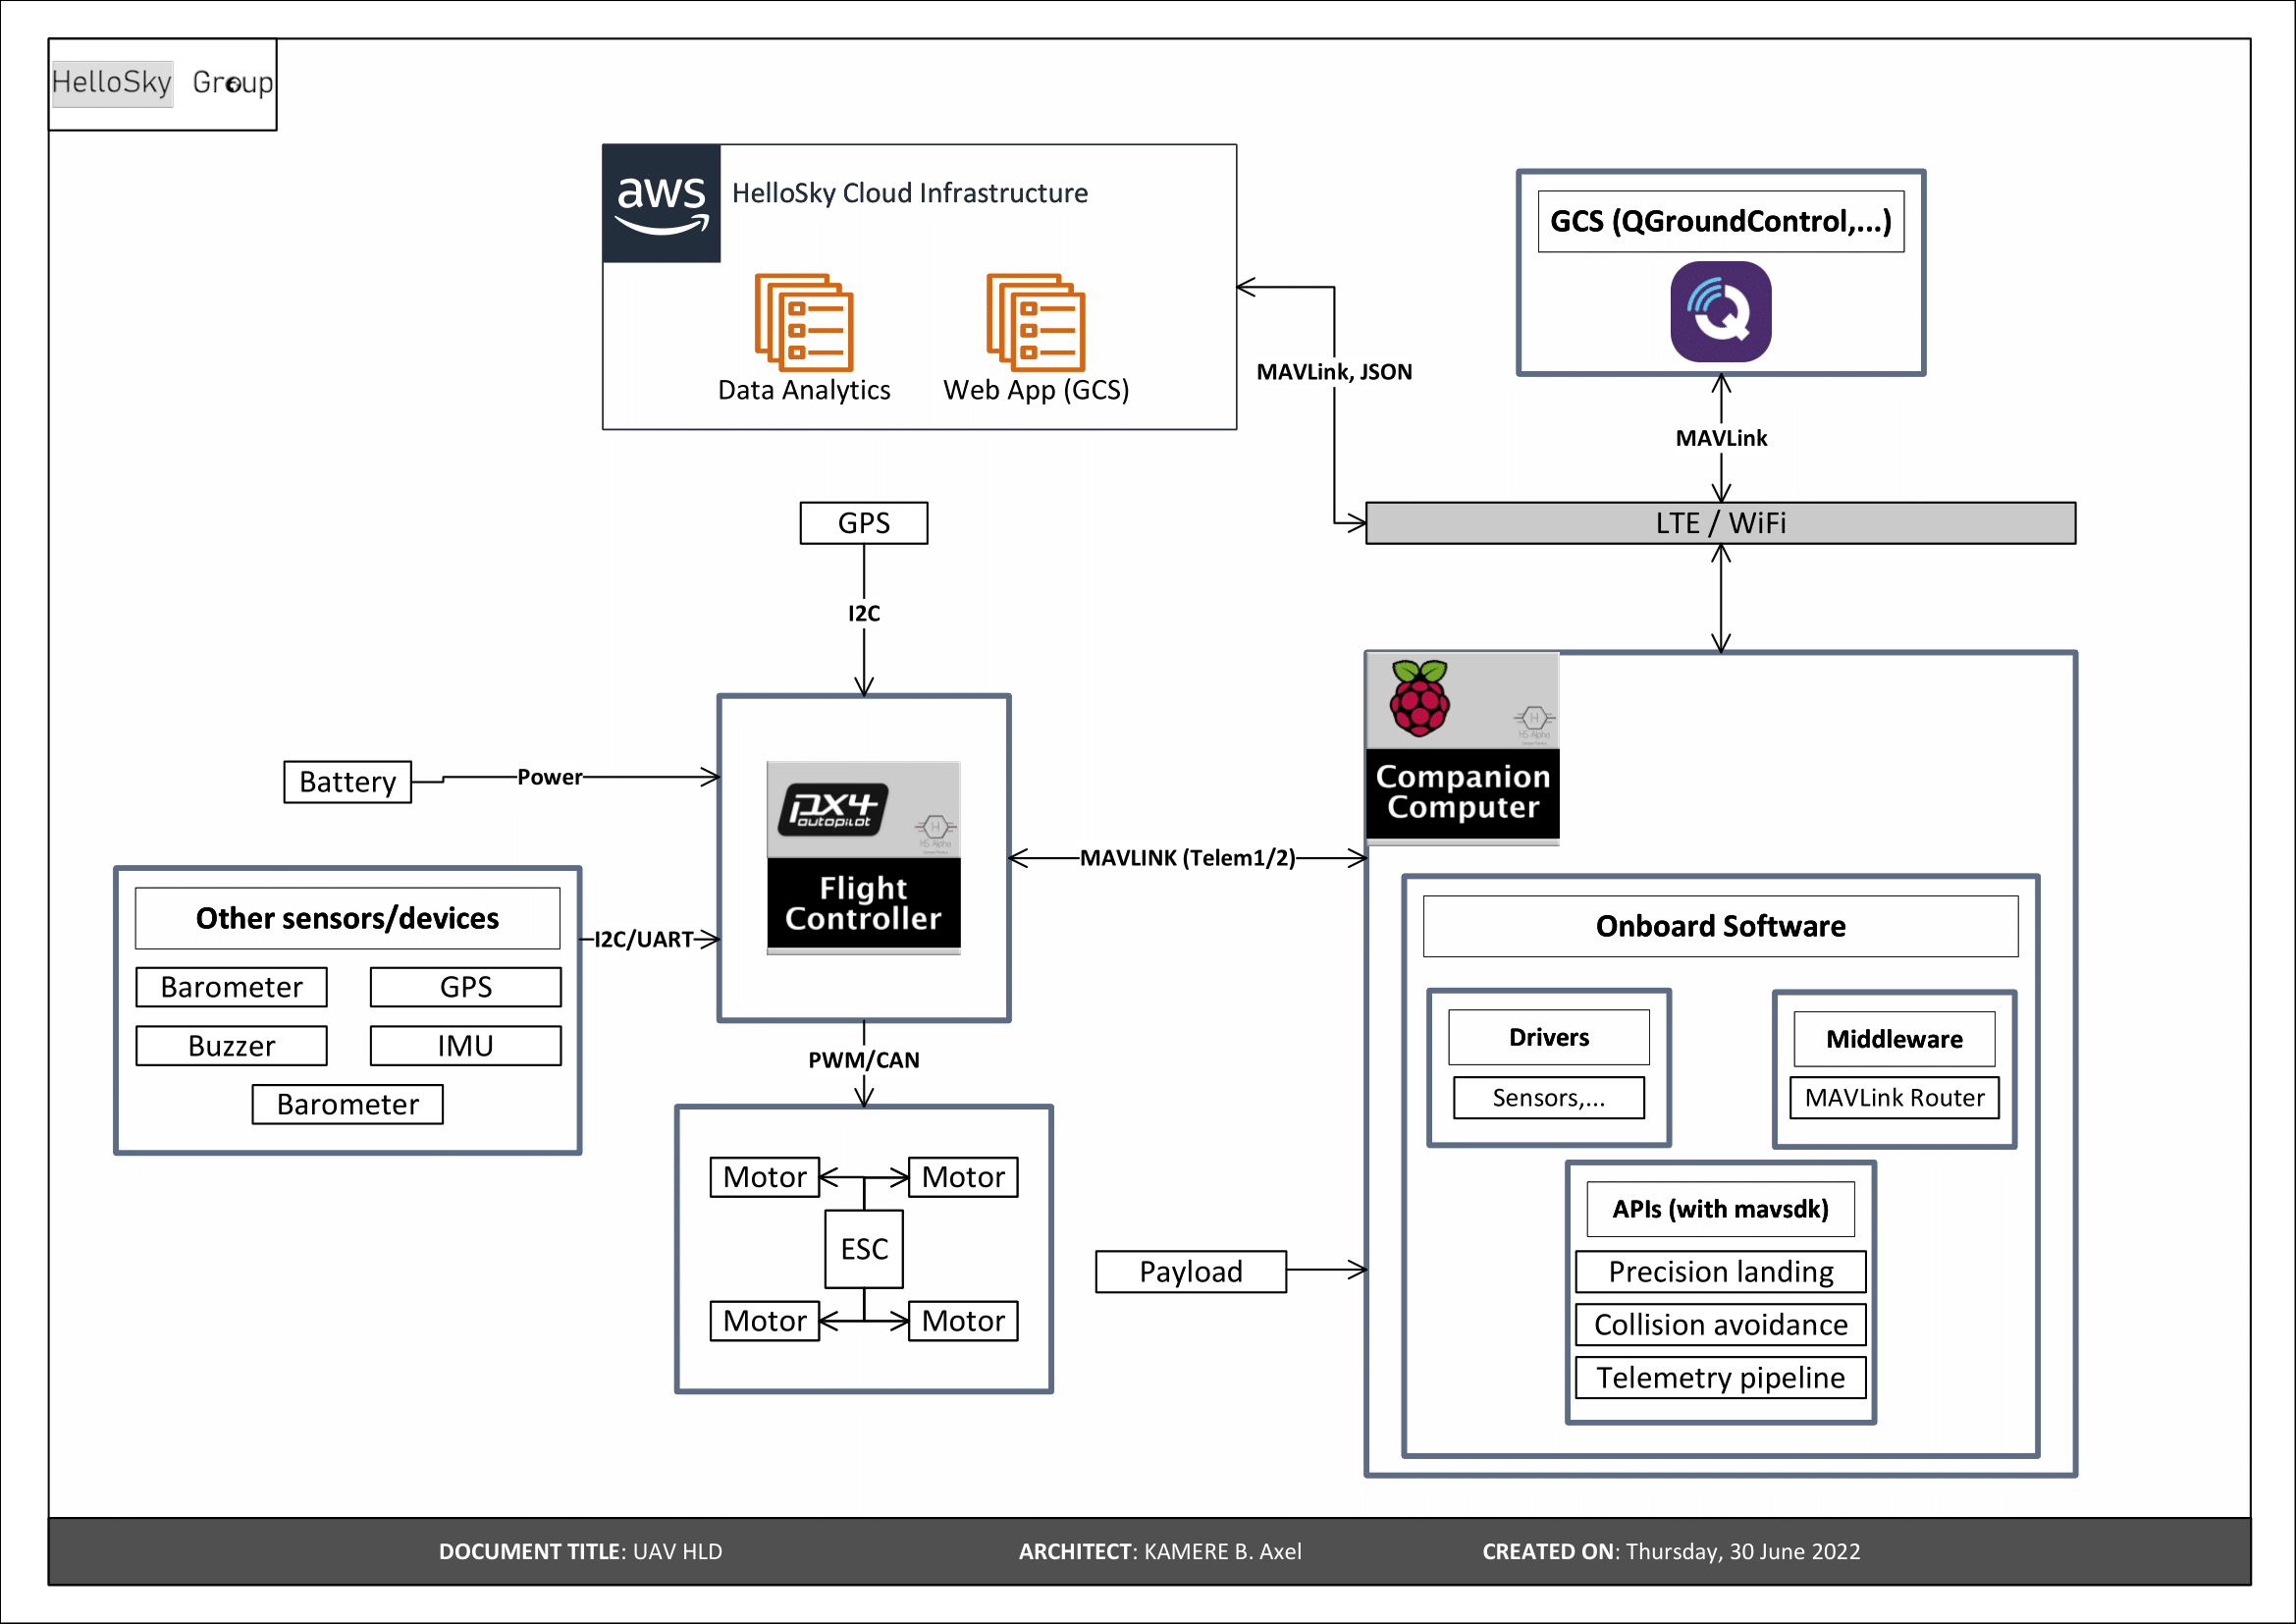
\includegraphics[width=1\linewidth]{uav_hld.png}
    \caption{Proposed unmanned aerial vehicle high-level design.}
    \label{fig:uav-hld}
    \source{Own work. Designed with Microsoft Visio. Refer to \ref{subsec:ms-visio}.}
\end{figure}

As one can see from the design, the proposed UAV comprises of about 5 main components. Starting from the top going clockwise they are:
\begin{itemize}
    \item A cloud infrastructure that hosts web app and data analytics services, where the UAV sends data and receives mission commands from.
    \item An on-premise ground control station where the UAV can also be controlled from.
    \item An LTE/WiFi module that establishes remote network connectivity.
    \item A companion computer. This hosts multiple software like drivers for various sensors that can be attached to the computer, middleware like the MAVLink router which allows MAVLink traffic to be routed to external destinations, and APIs built with various libraries like MAVSDK\cite{mavsdk} to enhance the UAV capability.
    \item A flight controller running PX4 firmware and is connected to various other components like the electronic speed controller (ESC), GPS, battery and other sensors or devices.
\end{itemize}

%/------------------------------- SUB-SECTION END -------------------------------/%


%/------------------------------ SUB-SECTION START ------------------------------/%

\subsection{Classification of Unmanned Aerial Vehicles}
\label{subsubsec:classification-of-uavs}

UAVs come in different classifications depending on various factors like weight and payload, application, wing and rotor shape, and operational range and altitude. There is no one standard used across the industry to identify UAVs.

%/---------------------------- SUB-SUB-SECTION START ----------------------------/%

\subsubsection*{Classification by operational altitude and range}

\begin{table}[H]
    \centering
    \begin{tabular}{|c|c|c|}
        \hline
        Type                                  & Altitude (km) & Range (km) \\
        \hline\hline
        Hand-held                             & <0.6          & <2         \\
        \hline
        Close                                 & <1.5          & <10        \\
        \hline
        NATO                                  & <3            & <50        \\
        \hline
        Tactical                              & <5.5          & <160       \\
        \hline
        Medium Altitude Long Endurance (MALE) & <9.1          & <200       \\
        \hline
        High Altitude Long Endurance (HALE)   & >9.1          & -          \\
        \hline
        Hypersonic                            & <15.2         & >200       \\
        \hline
    \end{tabular}
    \caption{UAV classification by altitude and range.}
    \source{Vinay et Al \cite{Chamola2021}}
    \label{table:uav-classification-by-alt-range}
\end{table}

%/----------------------------- SUB-SUB-SECTION END -----------------------------/%


%/---------------------------- SUB-SUB-SECTION START ----------------------------/%

\subsubsection*{Classification by application}

\begin{table}[H]
    \centering
    \begin{tabular}{|c|c|c|}
        \hline
        Type                                & Use cases                                 \\
        \hline\hline
        Personal                            & photography, entertainment                \\
        \hline
        Emergency units and Law Enforcement & search and rescue, patrolling             \\
        \hline
        Commercial                          & aerial imaging, delivery, site monitoring \\
        \hline
        Military                            & reconnaissance, attacks                   \\
        \hline
    \end{tabular}
    \caption{UAV classification by application and use case.}
    \source{Adapted from \cite{Chamola2021}}
    \label{table:uav-classification-by-application}
\end{table}

%/----------------------------- SUB-SUB-SECTION END -----------------------------/%


%/---------------------------- SUB-SUB-SECTION START ----------------------------/%

\subsubsection*{Classification by weight and payload}

\begin{table}[H]
    \centering
    \begin{tabular}{|c|c|c|}
        \hline
        Type   & Weight (Range, kg) \\
        \hline\hline
        Nano   & < 0.25             \\
        \hline
        Micro  & 0.25 - 2           \\
        \hline
        Small  & 2 - 25             \\
        \hline
        Medium & 25 - 150           \\
        \hline
        Large  & > 150              \\
        \hline
    \end{tabular}
    \caption{UAV classification by weight.}
    \source{Adapted from \cite{Chamola2021}}
    \label{table:uav-classification-by-weight}
\end{table}

%/----------------------------- SUB-SUB-SECTION END -----------------------------/%


%/---------------------------- SUB-SUB-SECTION START ----------------------------/%

\subsubsection*{Classification by wing and rotor shape}

<TODO: ATTACH IMAGE>
%/----------------------------- SUB-SUB-SECTION END -----------------------------/%

%/------------------------------- SUB-SECTION END -------------------------------/%

%/--------------------------------- SECTION END ---------------------------------/%


%/-------------------------------- SECTION START --------------------------------/%

\section{Amazon Web Services}
\label{sec:aws}

Amazon Web Services, commonly known as AWS, is a cloud platform provided by Amazon that provides various service offerings such as platform as a service, PaaS, and infrastructure as a service, IaaS\cite{awswhatisaws2022}. AWS makes it easy for developers, engineers and businesses to deploy scalable, resilient, agile and highly available infrastructures for databases, servers, applications, storage, analytics, \textit{et cetera}. AWS offers attractive and cost saving payment strategies of which there are pay-as-you-go, save when you commit, and pay less by using more\cite{awspricing2022}.

AWS has a concept of regions, which refers to a physical location around the world, where multiple data centres are deployed in a cluster. Each cluster of data centre is called an availability zone\cite{awsregionsandazs}. AWS set this up like this to guarantee high availability and reliability of deployed resources.

\begin{figure}[H]
    \centering 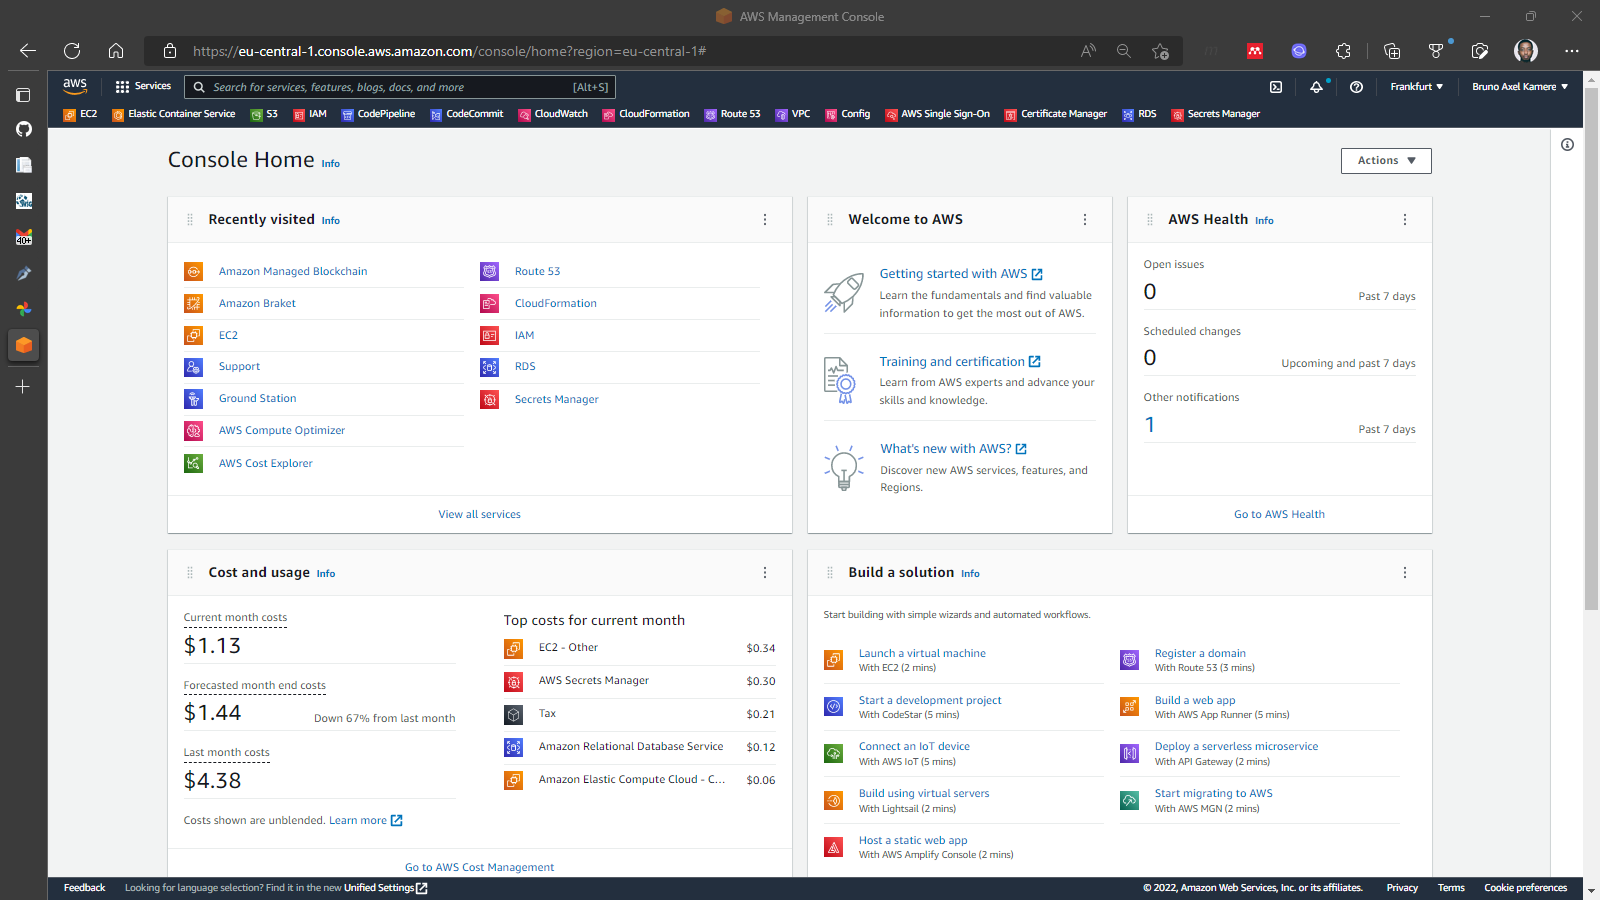
\includegraphics[width=0.9\linewidth]{aws_console_home.png}
    \caption{AWS console home.}
    \label{fig:aws-console-home}
    \source{Own work.}
\end{figure}

Cloud computing is an emerging technology that has revolutionized how businesses go online. Cloud computing has been and still is of great use in various industries, including the aerospace and energy industries. One of the many usage of cloud computing like AWS in the aerospace and energy industries is where Burak et al developed a cloud and edge solution running on AWS that aimed at increasing turbine maintenance inspections' efficiency through automation and a serverless AWS architecture while reducing operations cost\cite{burakawswindfarm2021}. The solution proposed by Burak et al was comprised of drones, machine learning and internet of things processes running on cloud and edge.

The proposed solution in this thesis also takes advantage of what AWS and cloud computing offers. Several components, like data analytics services, of the proposed solution are running on AWS. Figure \ref{fig:aws-architecture-hld} shows the AWS high-level design of the proposed solution. The details of the design are described in chapter \ref{chap:methodology-and-setup}.

% This image is already used in the solution description section
% \begin{figure}[H]
%     \centering 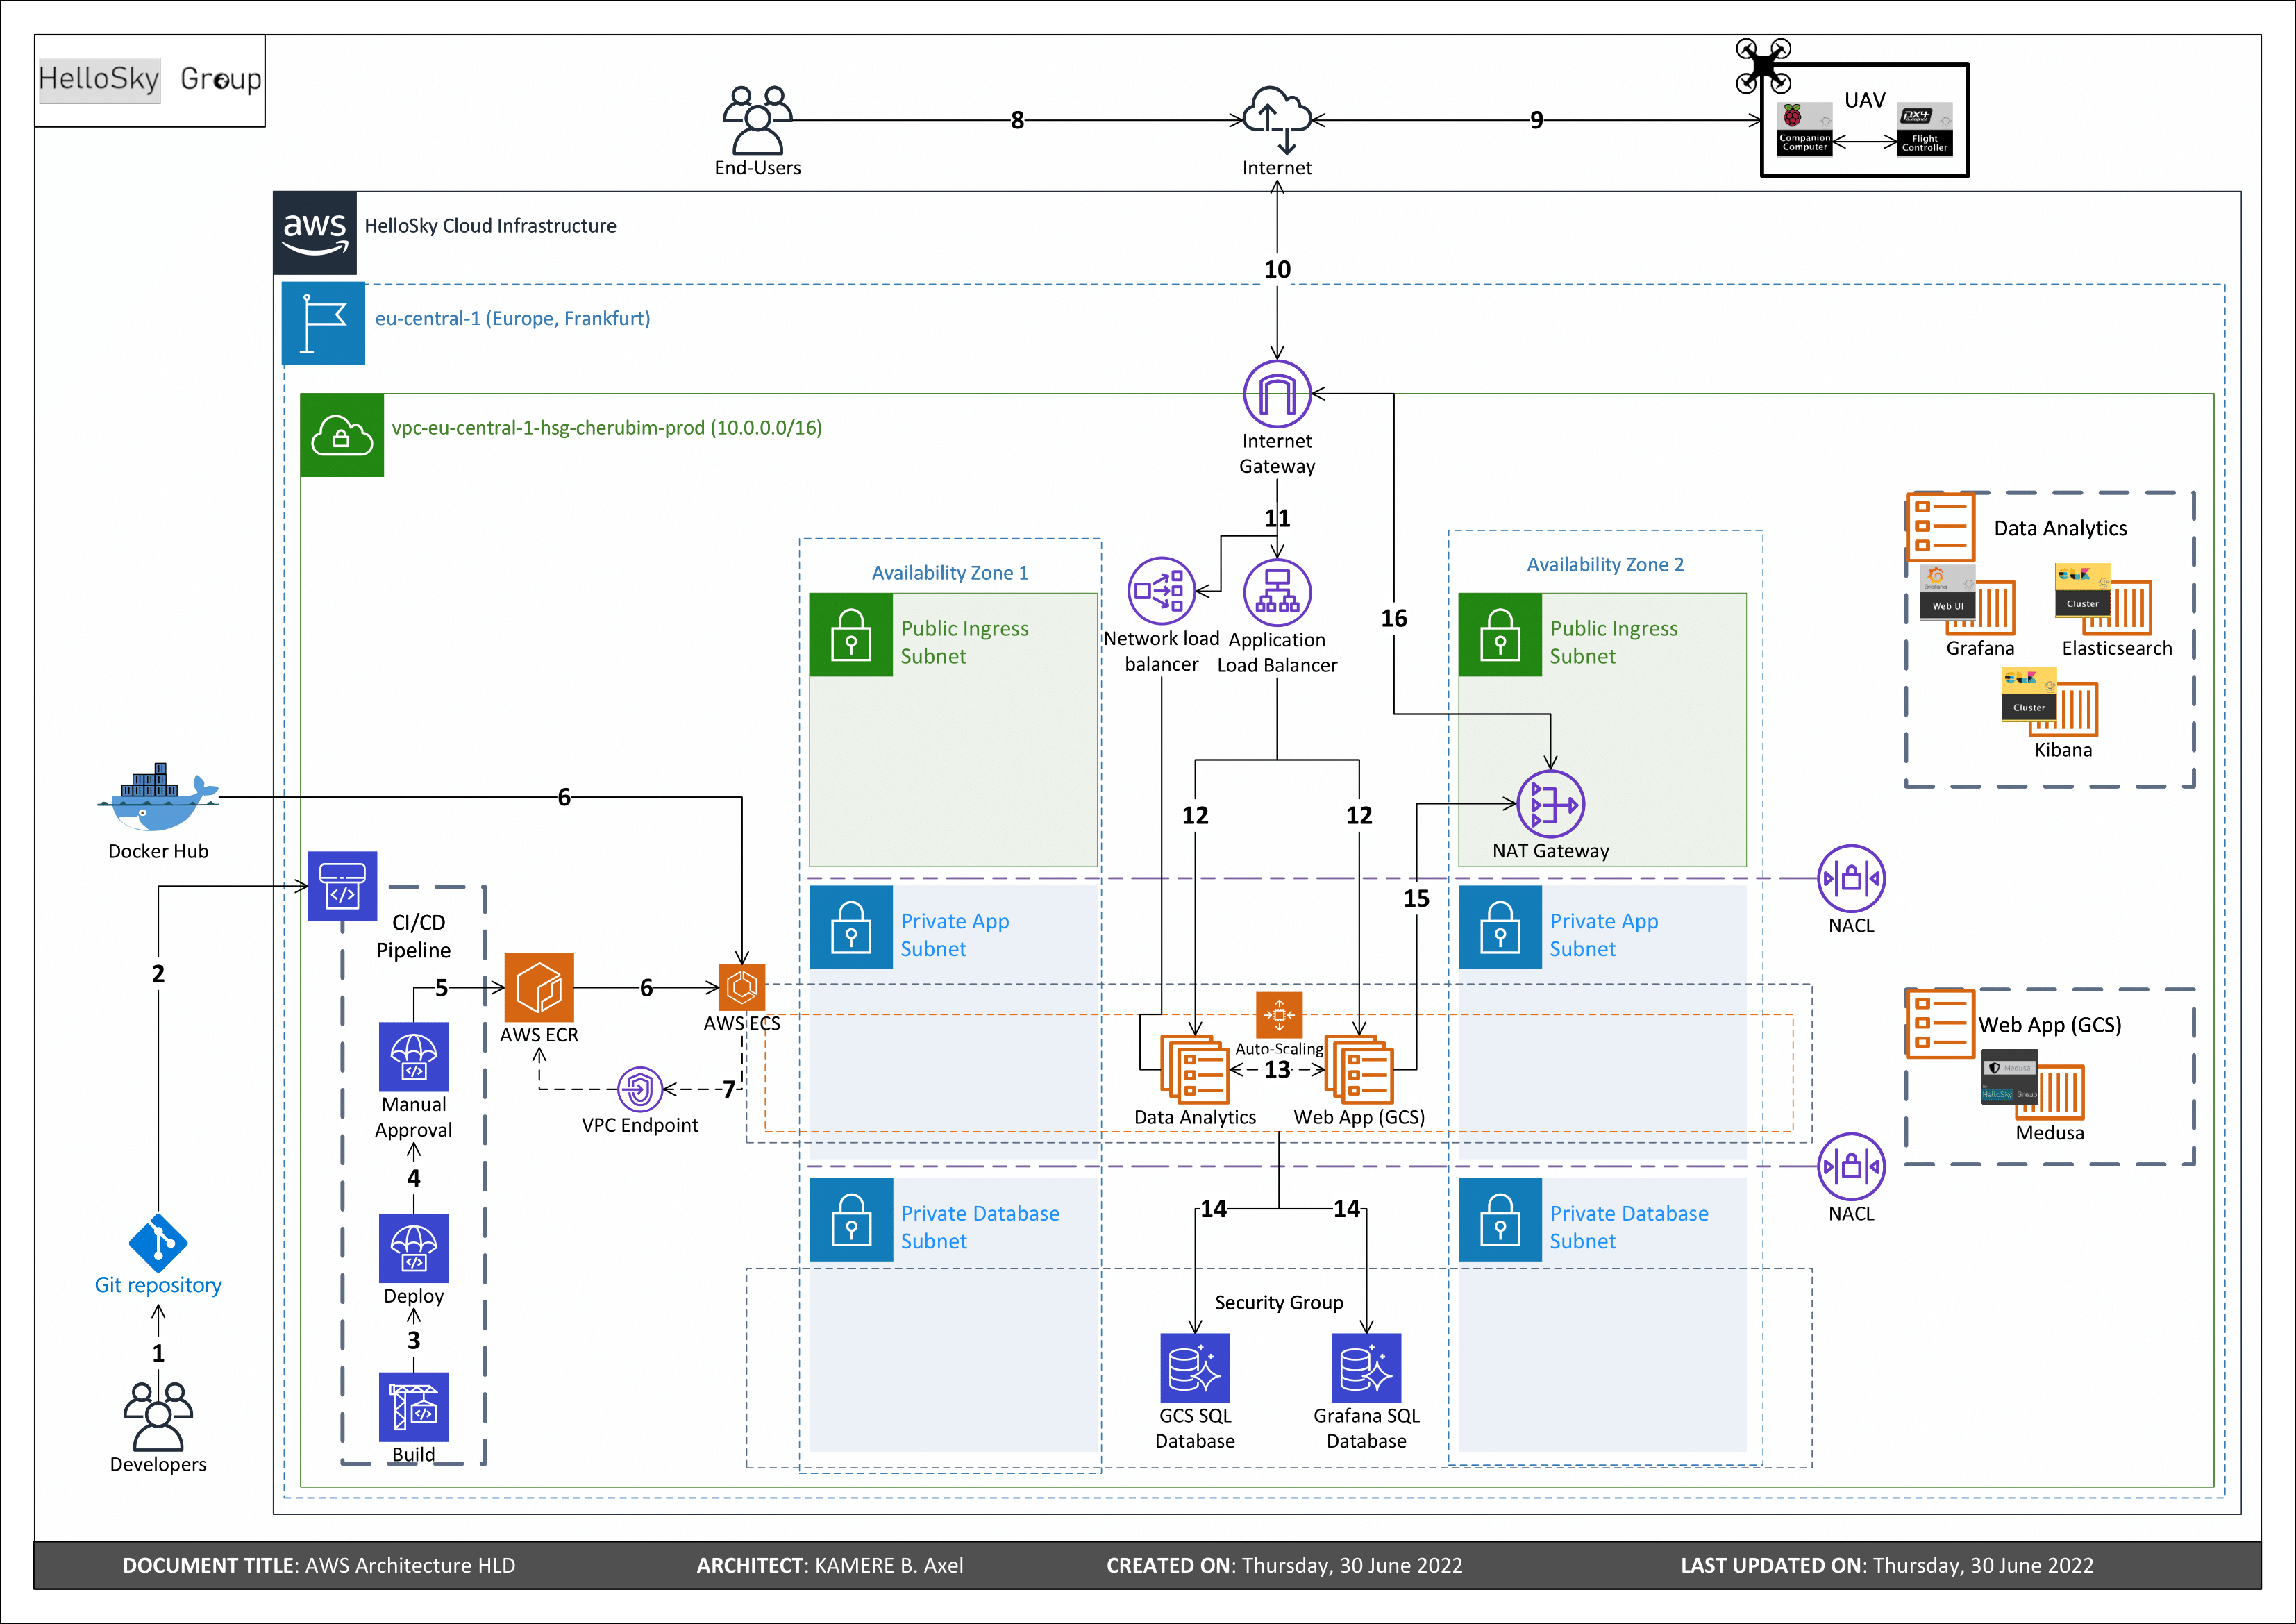
\includegraphics[width=1\linewidth]{aws_architecture_hld.png}
%     \caption{Proposed AWS architecture high-level design.}
%     \label{fig:aws-architecture-hld}
%     \source{Own work. Designed with Microsoft Visio. Refer to \ref{subsec:ms-visio}.}
% \end{figure}


%/------------------------------ SUB-SECTION START ------------------------------/%

\subsection{Infrastructure as code}
\label{subsec:iac}

Infrastructure as Code also known as IaC, a technique very often used in the DevOps and automation community, is an infrastructure that is provisioned through code and scripts usually written in familiar programming languages like Python, PHP, Node.JS, C\# \textit{et cetera}. The infrastructure deployed through code can be servers, databases, firewalls, full fledged data centres \textit{et cetera}. The main advantages of defining an infrastructure as code are:

\begin{itemize}
    \item Improved efficiency and consistency.
    \item Reduced human error.
    \item Infrastructure agility. An infrastructure defined as code can be deployed as many times as needed, which reduces the effort invested by developers in case a replica of an environment is needed elsewhere.
    \item It allows developers to take advantage of programming languages features like loops, variables \textit{et cetera} to build more agile infrastructures.
    \item The infrastructure can be versioned and tightly controlled. Since the infrastructure is basically standard code, it can be versioned with various versioning tools like Git or Subversion. This facilitates maintenance and makes the infrastructure easy to be rolled back, in case of issues.
    \item It helps with cost savings. Since the whole infrastructure is basically deployed automatically through code, engineers can then shift their focus to work on other important tasks.
\end{itemize}

In this thesis, Infrastructure as Code is used to its outmost potential. The AWS infrastructure is deployed as code using the AWS proprietary software development framework called AWS Cloud Development Kit or AWS CDK. AWS CDK is an open source kit provided by AWS that allows engineers to define IT infrastructures on AWS using familiar programming languages. In the source code \ref{code:route_53_records} is an example snippet from the AWS CDK app developed for the proposed solution in this thesis. The snippet represents a part that adds DNS records to the AWS Route 53 service using standard Python code. Once the AWS CDK is deployed, the script will automatically create the resources defined in the AWS Route 53 DNS service.

\begin{center}
    \captionsetup{type=listing}
    \inputminted[
        frame=single,
        framesep=2mm,
        baselinestretch=1.2,
        fontsize=\footnotesize,
        breaklines,
        breakanywhere,
        linenos
    ]{python}{config/code/7c11d95d3b55be021475679db7f9f9dd/route_53_records.py}
    \captionof{listing}{helloskygroup.com AWS CDK Python Route 53 snippet.}
    \label{code:route_53_records}
\end{center}

%/------------------------------- SUB-SECTION END -------------------------------/%

%/--------------------------------- SECTION END ---------------------------------/%


%/-------------------------------- SECTION START --------------------------------/%

\section{Simulation}
\label{sec:simulation}

The proposed solution is designed based on actual physical hardware components, but during development phases, it usually is better to simulate parts of the solutions that can be simulated. This not only saves time, since everything is done through software, but it also saves money in case something initial project plan was to develop a whole UAS from scratch with an actual physical UAV and components, but this was deemed to be time consuming, and expensive to develop. During development of the proposed solution a simulation technique called Software-In-The-Loop or SITL\cite{Giese2021} was used to simulate the UAV. Figure \ref{fig:sitl-hld} shows the design of the proposed SITL architecture. Chapter \ref{chap:methodology-and-setup} elaborates more on this simulation technique. This technique basically allows developers to develop UAV flight logics using software and no hardware involved, eventhough it is possible as well to involve hardware in what is referred to as Hardware-In-The-Loop or HITL\cite{px4hitluserguide}. Chapter \ref{chap:methodology-and-setup} elaborates more on how SITL was used in this project to simulate an actual UAV with telemetry.

\begin{figure}[H]
    \centering 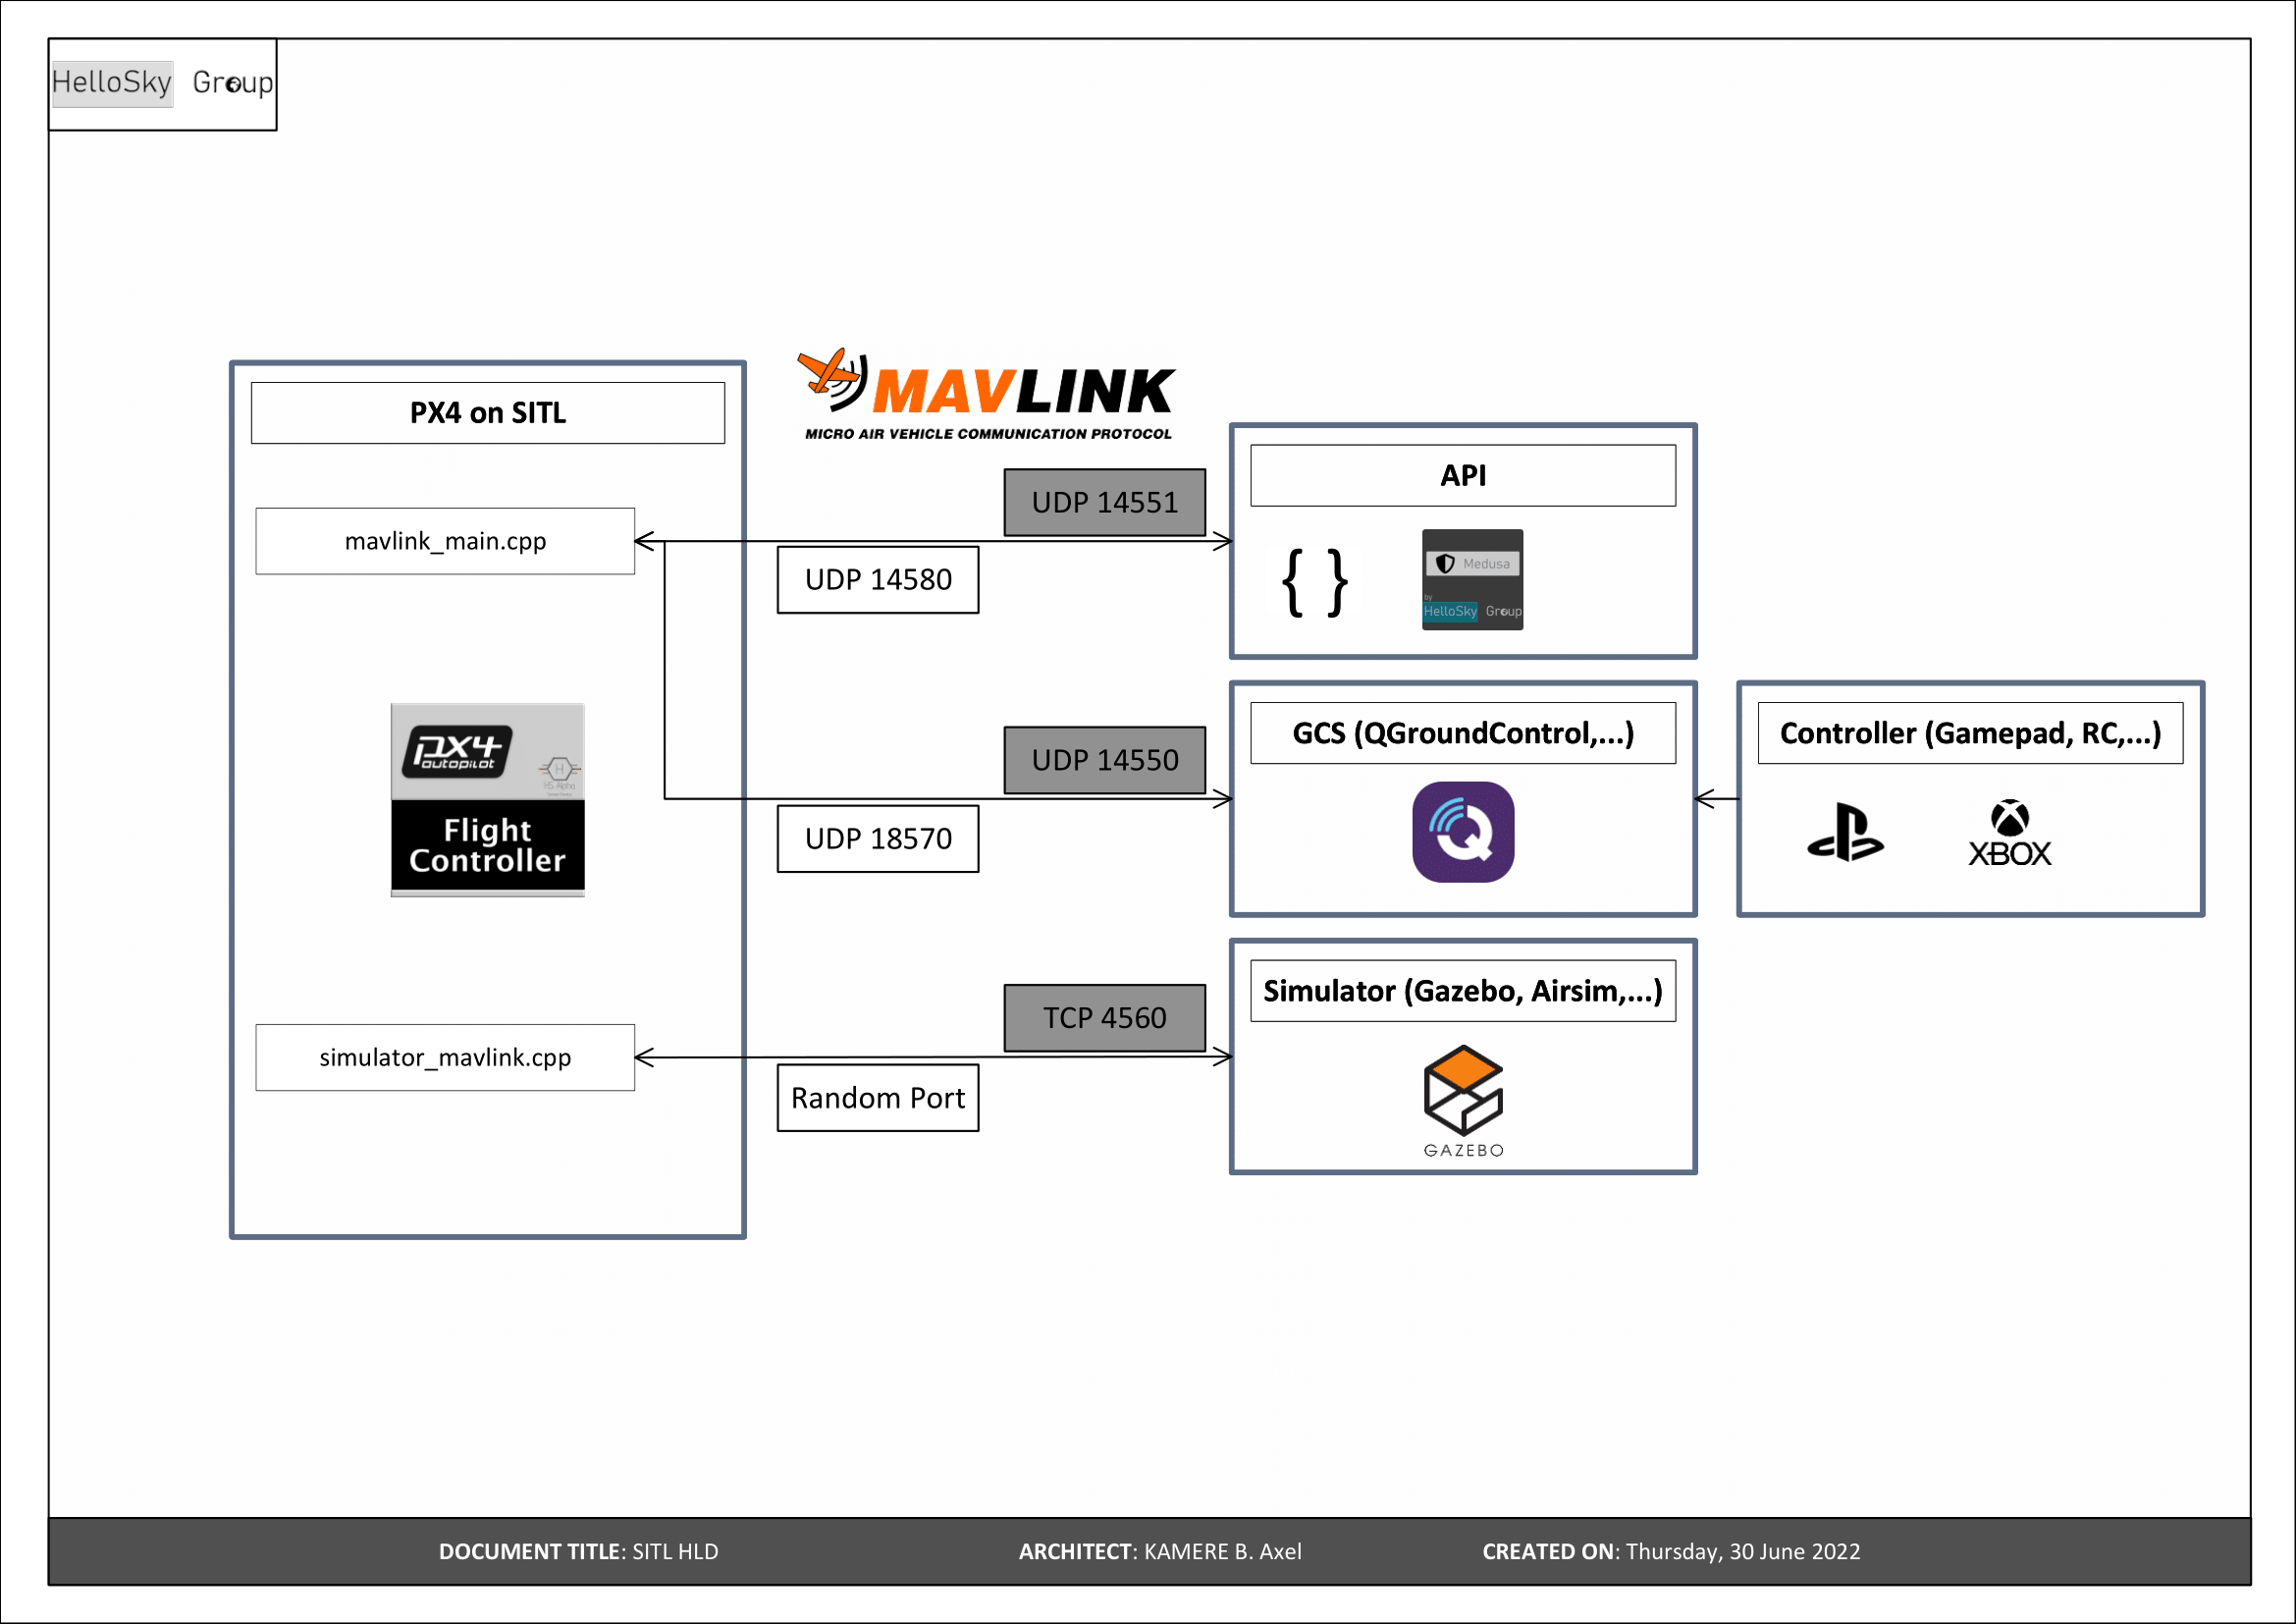
\includegraphics[width=1\linewidth]{sitl_hld.png}
    \caption{Proposed Simulation-In-The-Loop (SITL) architecture high-level design.}
    \label{fig:sitl-hld}
    \source{Own work. Designed with Microsoft Visio. Refer to \ref{subsec:ms-visio}.}
\end{figure}

%/--------------------------------- SECTION END ---------------------------------/%


%/-------------------------------- SECTION START --------------------------------/%

\section{Tools used}
\label{sec:tools-used}

The solution proposed in this thesis was built using various software development, and design tools. The choice of tools was really key to designing and developing an organised and consistent solution, therefore it was important to choose the right tools for the right tasks to help get the expected outcome.

In the next subsections, various used tools during the solution development are going to be listed and discussed.


%/------------------------------ SUB-SECTION START ------------------------------/%

\subsection{Microsoft visual studio code}
\label{subsec:ms-visual-studio-code}

Visual studio code or VS code is a source code editor provided by Microsoft. It was used in this thesis as a code editor to write various codes and scripts. VS code is a jack of all trades in a sense that it supports very well multiple programming languages, and since this project was comprised of multiple stacks of programming languages, VS code helped a lot during development.

\begin{figure}[H]
    \centering 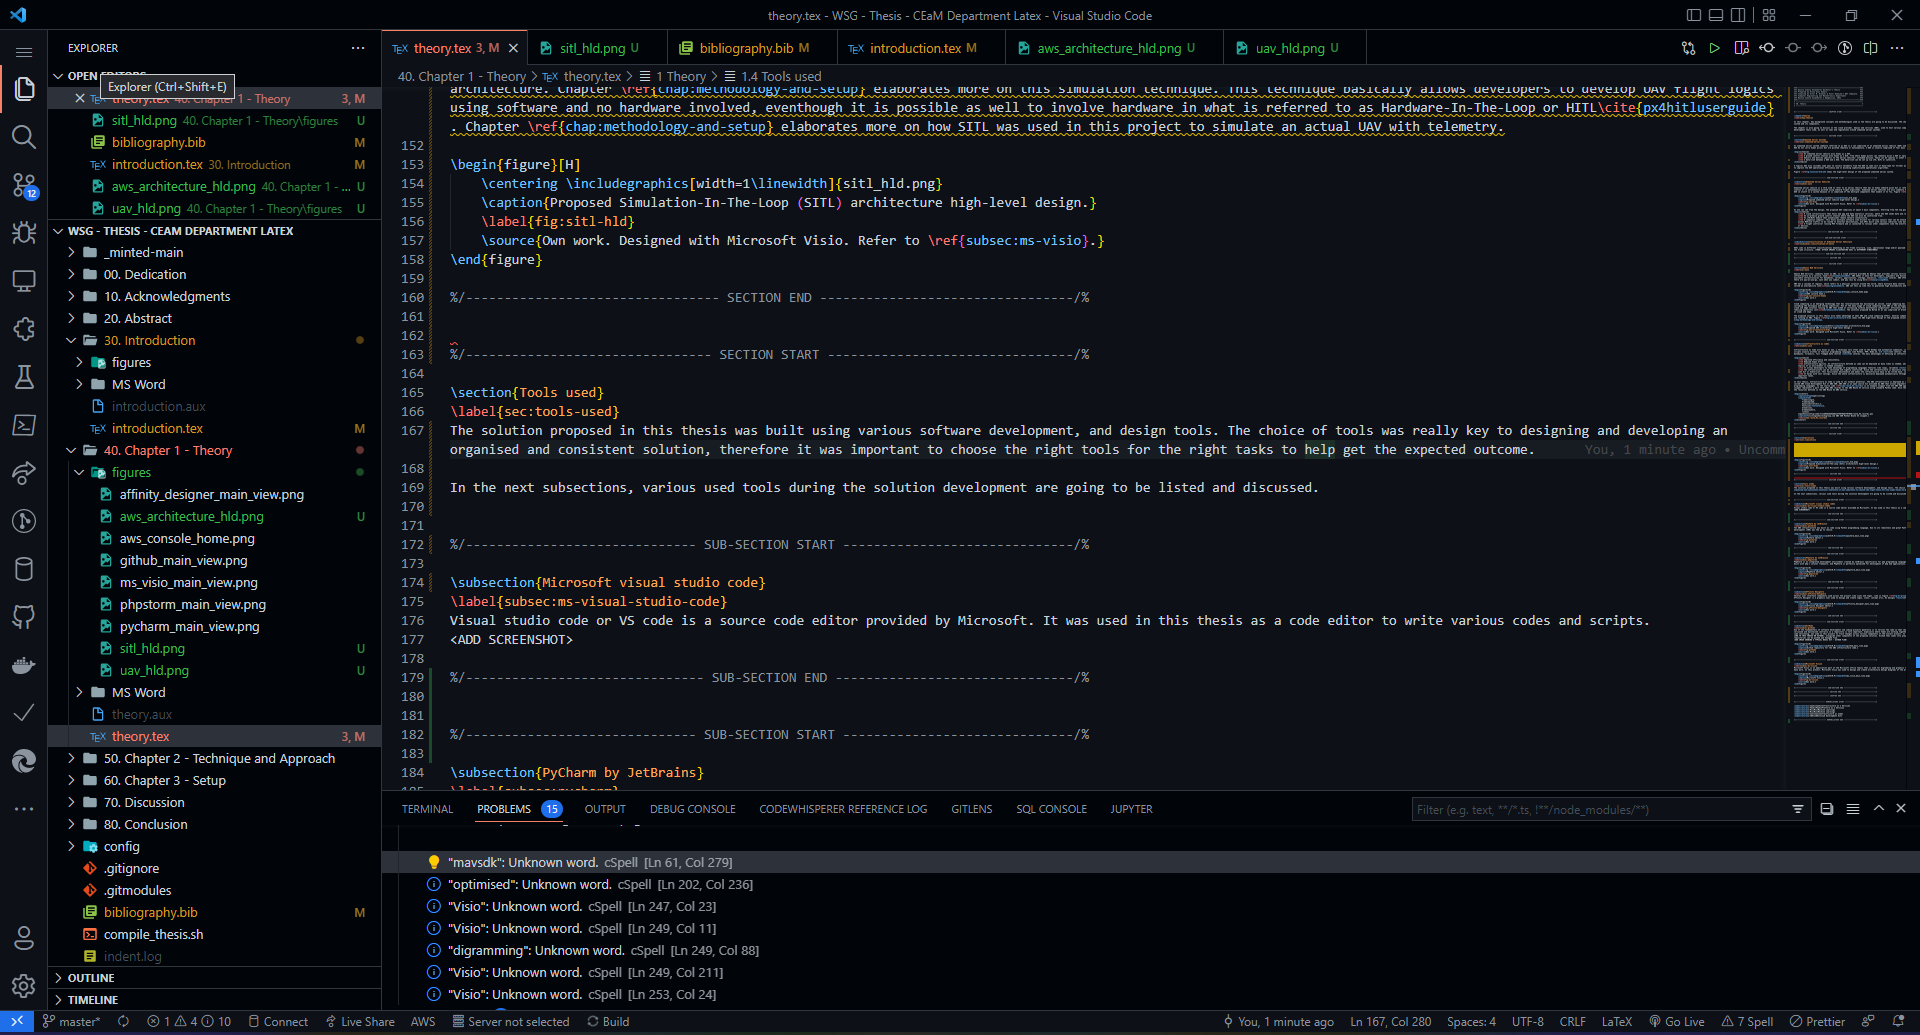
\includegraphics[width=0.9\linewidth]{ms_vs_code_main_view.png}
    \caption{Microsoft visual studio code editor.}
    \label{fig:ms-vs-code}
    \source{Own work.}
\end{figure}

%/------------------------------- SUB-SECTION END -------------------------------/%


%/------------------------------ SUB-SECTION START ------------------------------/%

\subsection{PyCharm by JetBrains}
\label{subsec:pycharm}

The AWS infrastructure was built as code using Python programming language. Due to its robustness and great Python support, Pycharm by JetBrains integrated development development (IDE) was the go to choice for Python code development.

\begin{figure}[H]
    \centering 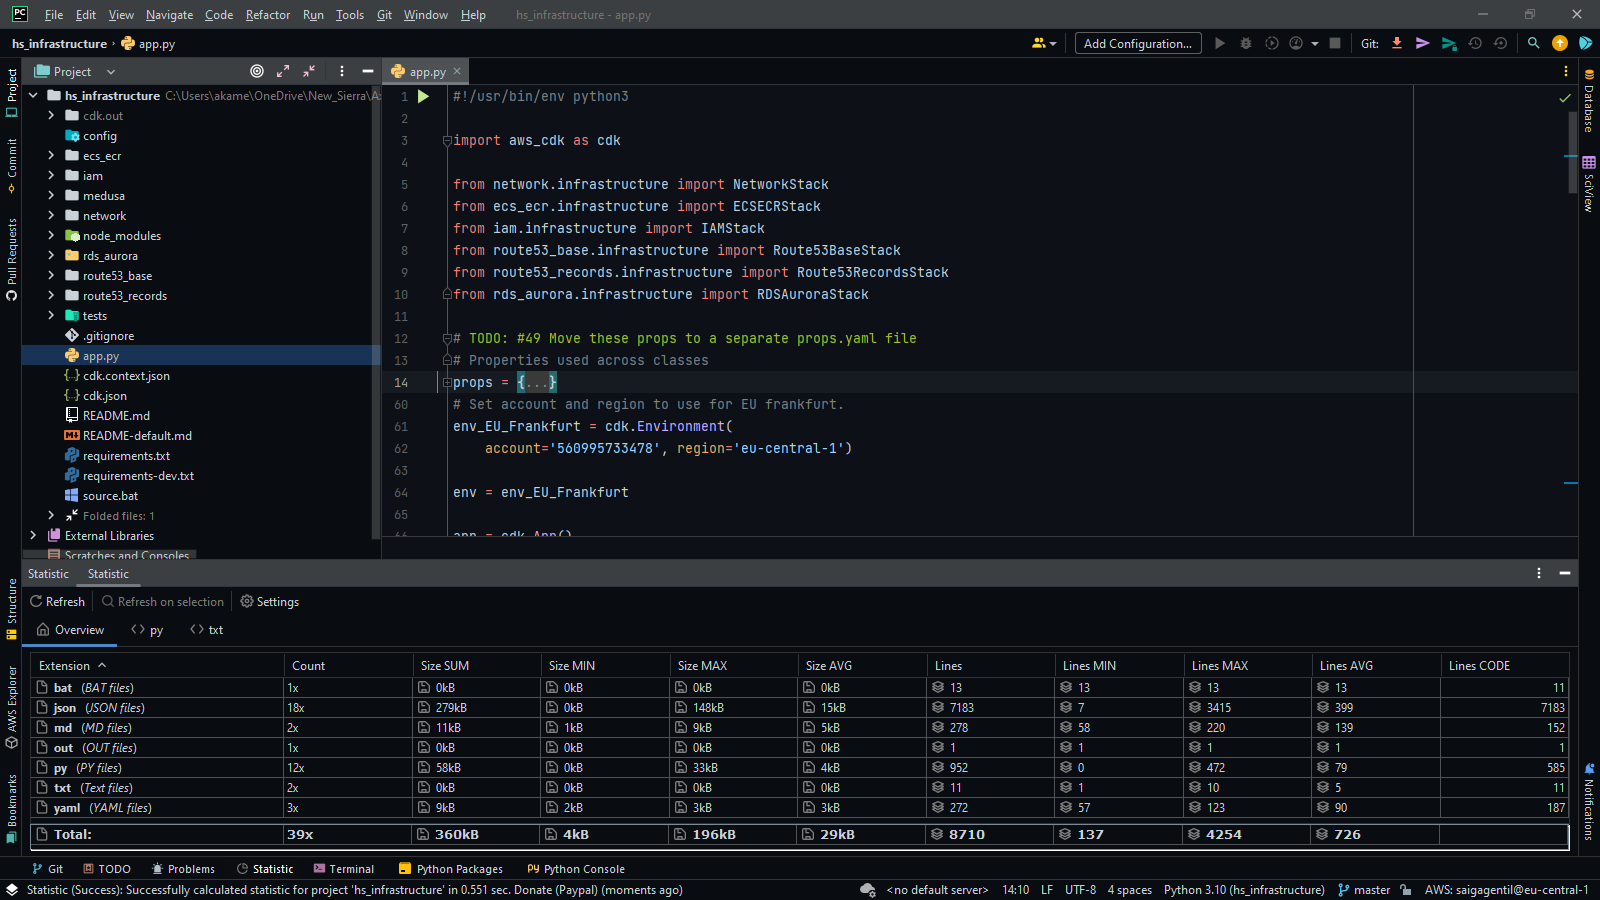
\includegraphics[width=0.9\linewidth]{pycharm_main_view.png}
    \caption{PyCharm editor.}
    \label{fig:pycharm}
    \source{Own work.}
\end{figure}

%/------------------------------- SUB-SECTION END -------------------------------/%


%/------------------------------ SUB-SECTION START ------------------------------/%

\subsection{PhpStorm by JetBrains}
\label{subsec:phpstorm}

PhpStorm is an integrated development environment created by JetBrains specifically for php programming language. The proposed web interface from which the UAV is controlled from is built with php's Laravel framework, and PhpStorm is perfectly optimised for development of php web applications.

\begin{figure}[H]
    \centering 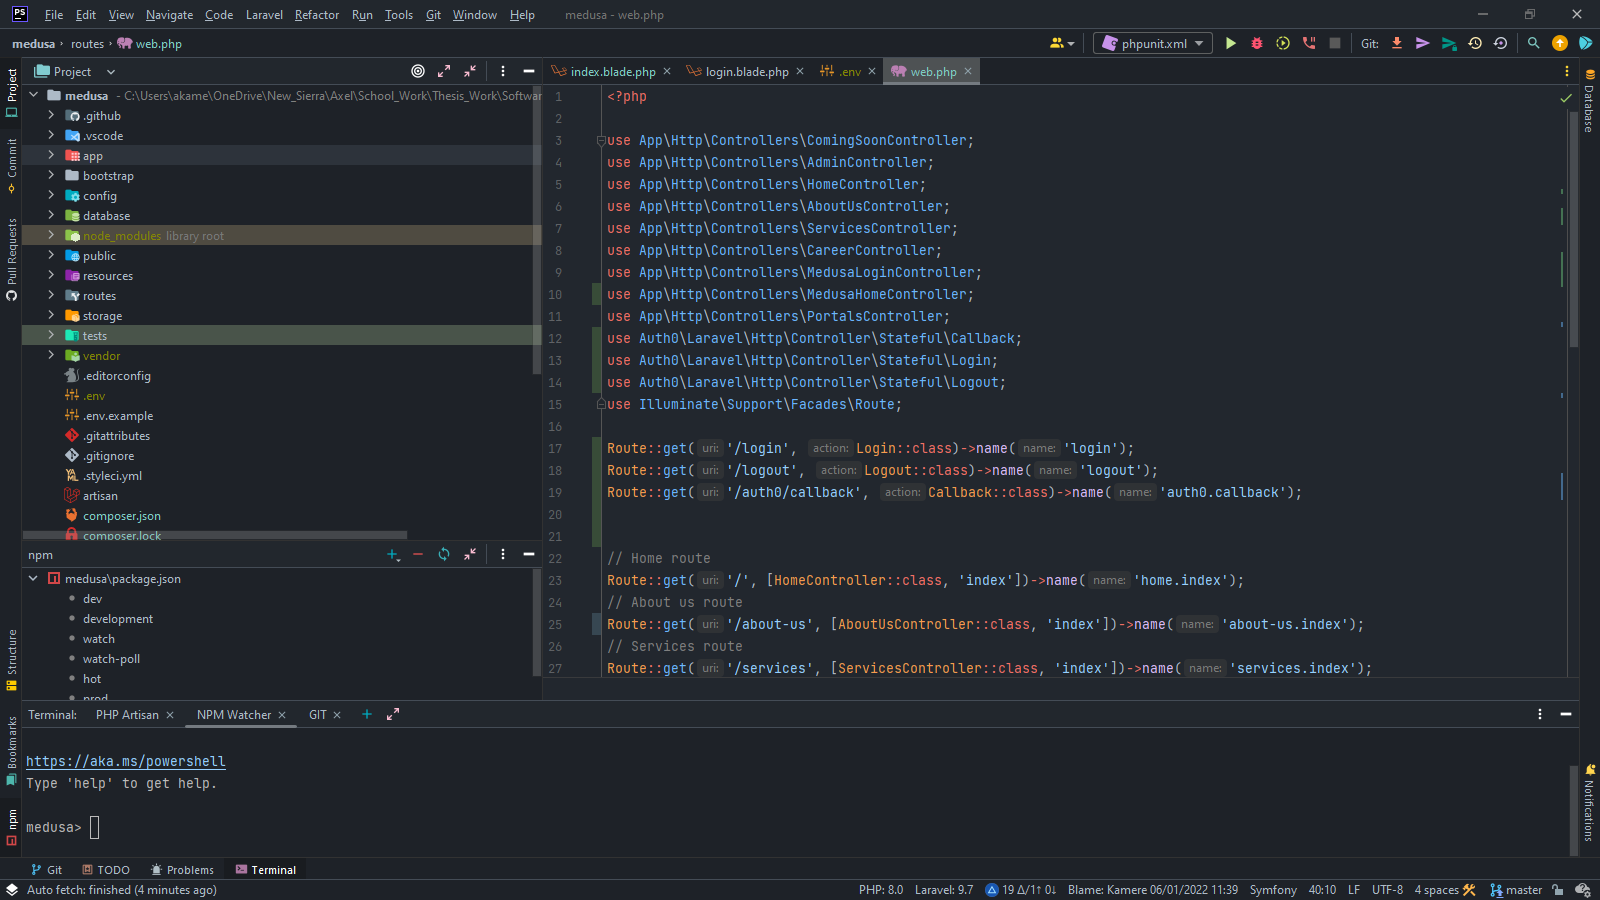
\includegraphics[width=0.9\linewidth]{phpstorm_main_view.png}
    \caption{PhpStorm editor.}
    \label{fig:phpstorm}
    \source{Own work.}
\end{figure}

%/------------------------------- SUB-SECTION END -------------------------------/%


%/------------------------------ SUB-SECTION START ------------------------------/%

\subsection{Affinity Designer}
\label{subsec:affinity-designer}

Several user interface components used across the project like icons and logos, like in figure \ref{fig:hs-group-logos} for example, were designed using Affinity Designer. Affinity Designer is a graphics tool used to design and create logos, icons, concept arts, UI designs \textit{et cetera}.

\begin{figure}[H]
    \centering 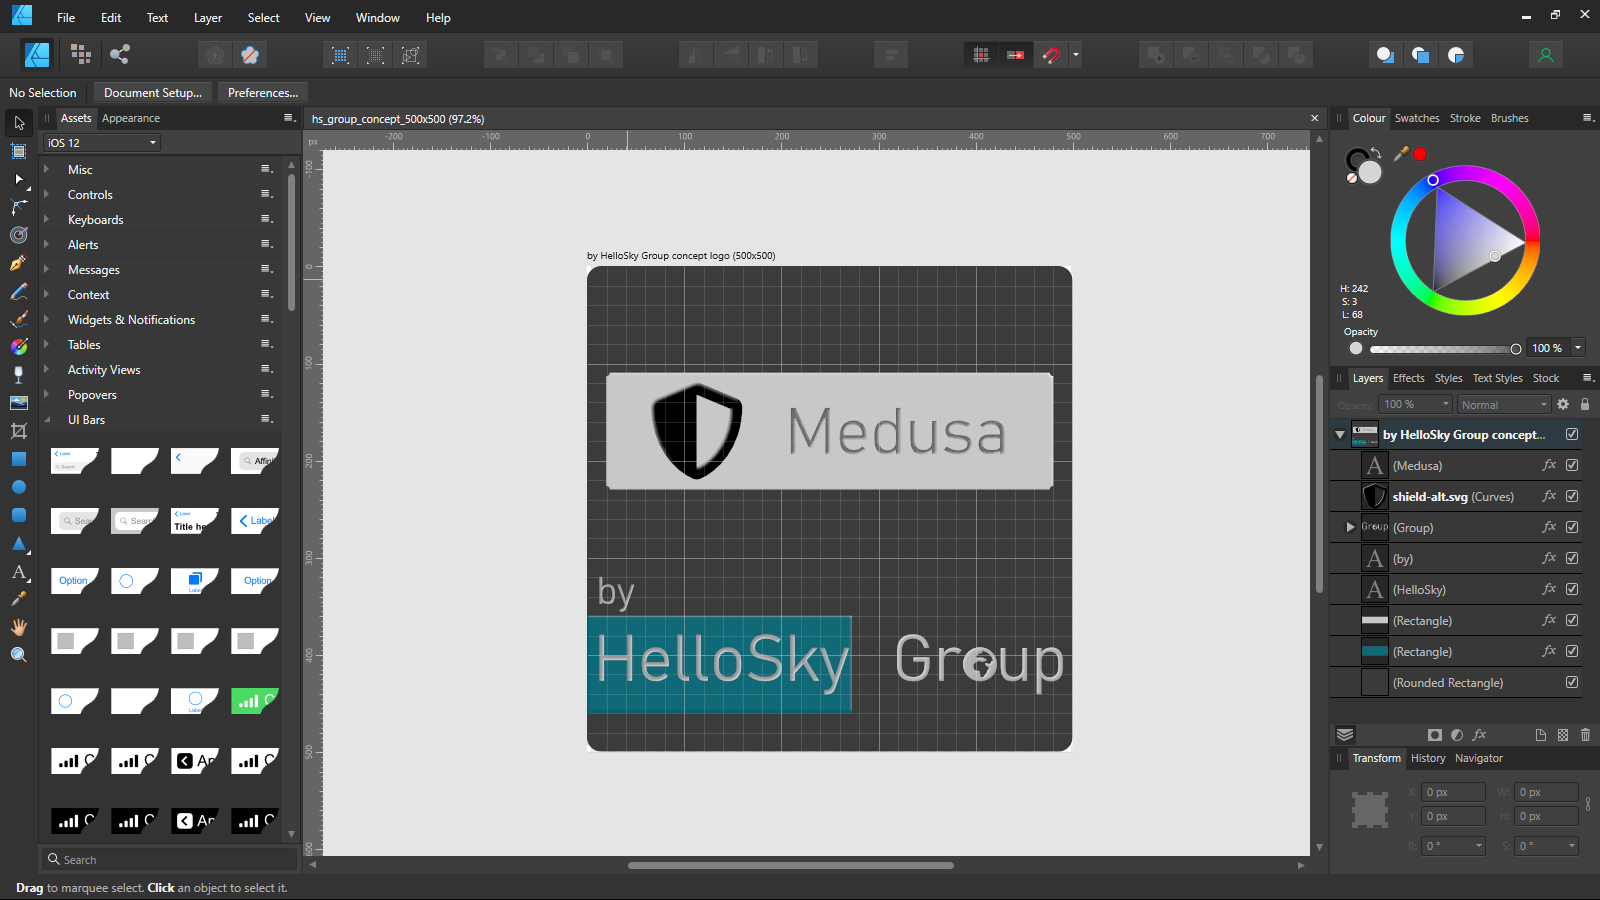
\includegraphics[width=0.9\linewidth]{affinity_designer_main_view.png}
    \caption{Affinity Designer editor.}
    \label{fig:affinity-designer}
    \source{Own work.}
\end{figure}

%/------------------------------- SUB-SECTION END -------------------------------/%


%/------------------------------ SUB-SECTION START ------------------------------/%

\subsection{GitHub}
\label{subsec:github}

One of the fundamentals of software development and coding projects generally is to version the code so that changes can be tracked overtime. Making sure that a project is versioned and maintained centrally in a repository is very important, especially where teams are working together on a similar project. Git, one of the softwares used for code versioning, was used in this project to track changes across various components of the overall project. In fact this thesis document itself is versioned with Git, alongside other components of the proposed solution. Github then comes into play to act as the single point of truth where multiple Git repositories can be pushed and managed from.

\begin{figure}[H]
    \centering 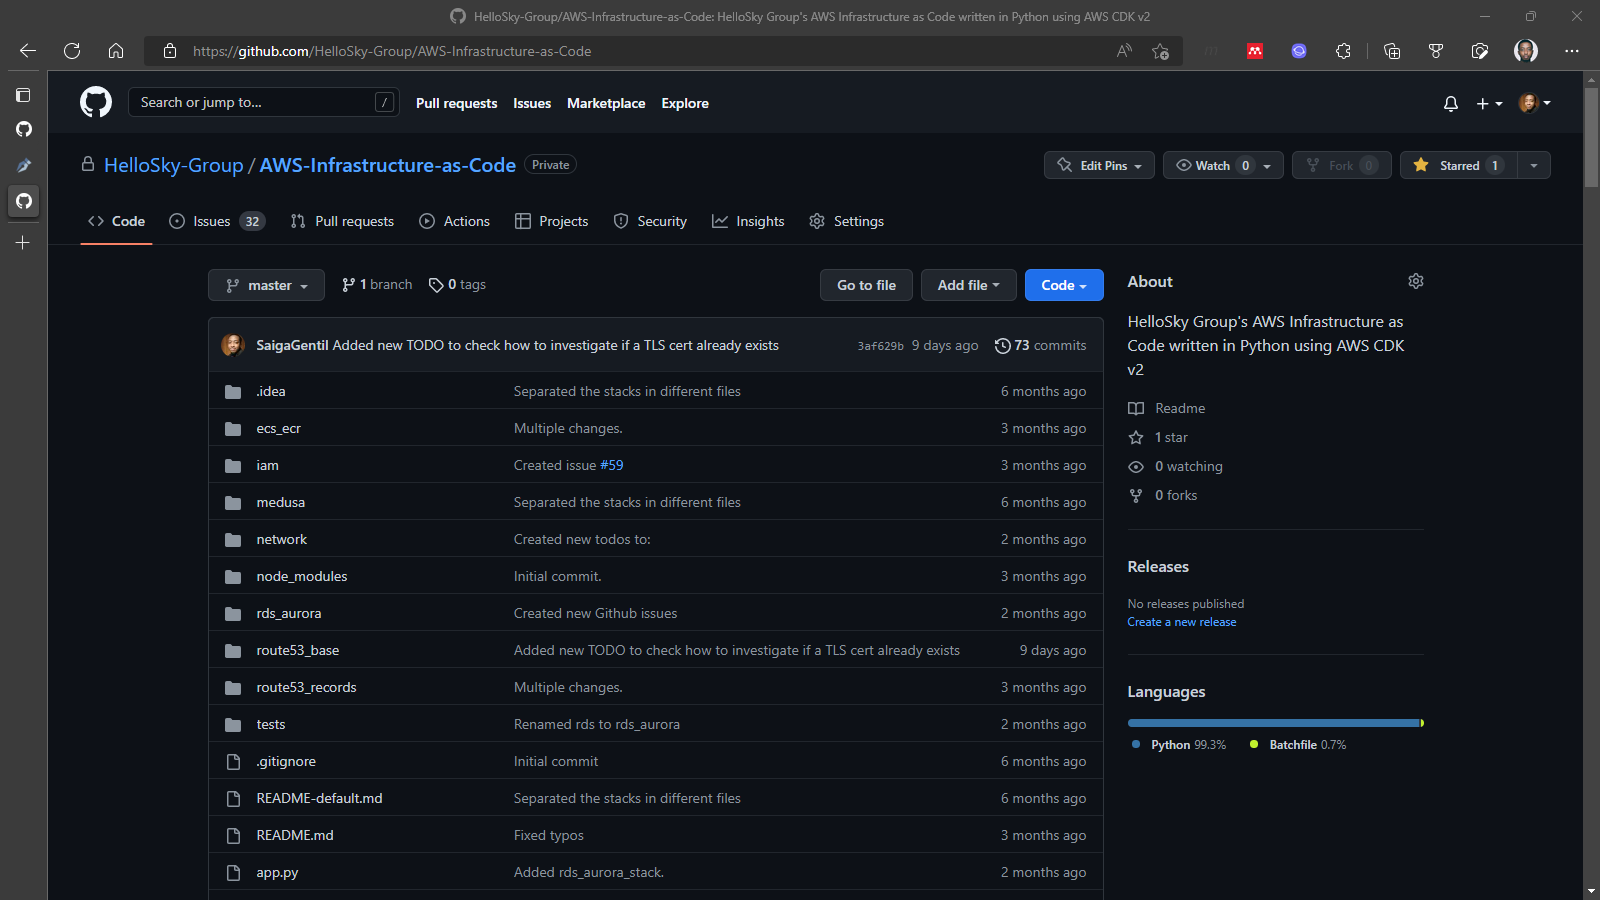
\includegraphics[width=0.9\linewidth]{github_main_view.png}
    \caption{Github repository for the AWS infrastructure code.}
    \label{fig:github}
    \source{Own work.}
\end{figure}


%/------------------------------ SUB-SECTION START ------------------------------/%

\subsection{Microsoft Visio}
\label{subsec:ms-visio}

Microsoft Visio is an application part of the Microsoft office family that is used for diagramming and graphics visualization. It is used to build architecture diagrams and many more. In this project, Microsoft Visio was used to design and create architecture design diagrams of the proposed solution.

\begin{figure}[H]
    \centering 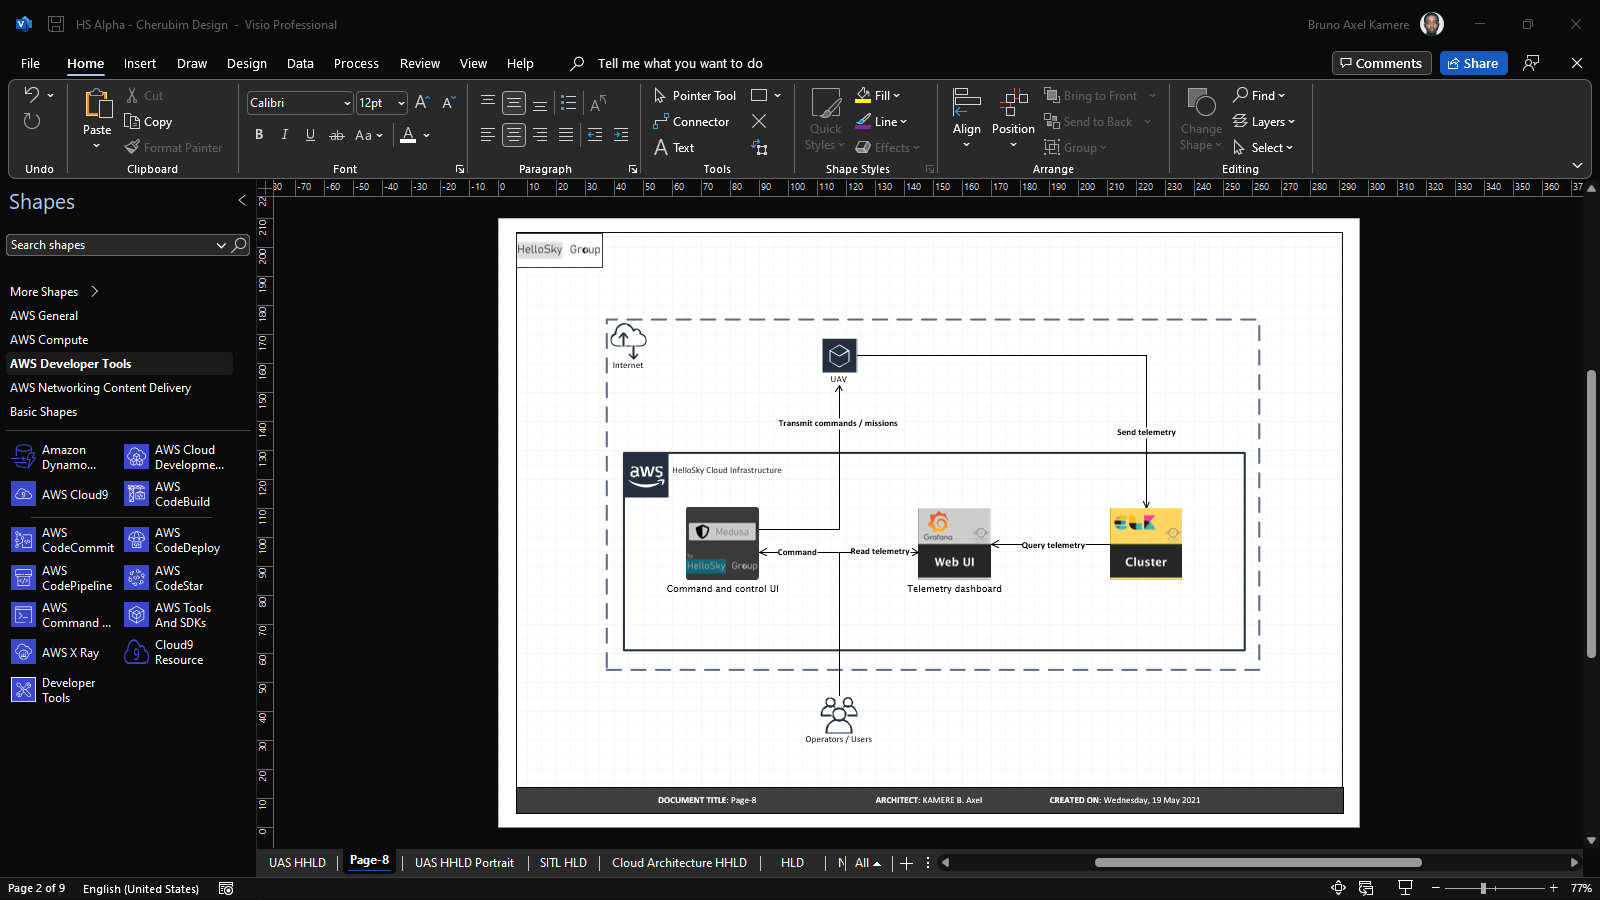
\includegraphics[width=0.9\linewidth]{ms_visio_main_view.png}
    \caption{Microsoft Visio.}
    \label{fig:ms-visio}
    \source{Own work.}
\end{figure}

%/------------------------------- SUB-SECTION END -------------------------------/%

%/--------------------------------- SECTION END ---------------------------------/%

%/--------------------------------- CHAPTER END ---------------------------------/%


%/----------------------------- NOMENCLATURE START ------------------------------/%

\nomenclature[z-IaaS]{IaaS}{Infrastructure as a Service}
\nomenclature[z-PaaS]{PaaS}{Platform as a Service}
\nomenclature[z-ML]{ML}{Machine Learning}
\nomenclature[z-ML]{ML}{Machine Learning}
\nomenclature[z-IaC]{IaC}{Infrastructure as Code}
\nomenclature[z-CDK]{CDK}{Cloud Development Kit}
\nomenclature[z-HITL]{HITL}{Hardware In The Loop}
\nomenclature[z-SITL]{SITL}{Software In The Loop}
\nomenclature[z-MAVLink]{MAVLink}{Micro Air Vehicle Link}
\nomenclature[z-MAVSDK]{MAVSDK}{Micro Air Vehicle Software Development Kit}
\nomenclature[z-KG]{KG}{Kilo Grams}
\nomenclature[z-KM]{KM}{Kilo Meters}

%/------------------------------ NOMENCLATURE END -------------------------------/%
